\documentclass[11pt]{scrartcl}

\usepackage{biblatex}
\usepackage{graphicx}
\usepackage{float}
\usepackage{listings}
\usepackage{booktabs}
\usepackage[utf8]{inputenc}

% Copyright 2017 Sergei Tikhomirov, MIT License
% https://github.com/s-tikhomirov/solidity-latex-highlighting/

\usepackage{listings, xcolor}

\definecolor{verylightgray}{rgb}{.97,.97,.97}

\lstdefinelanguage{Solidity}{
	keywords=[1]{anonymous, assembly, assert, balance, break, call, callcode, case, catch, class, constant, continue, contract, debugger, default, delegatecall, delete, do, else, event, export, external, false, finally, for, function, gas, if, implements, import, in, indexed, instanceof, interface, internal, is, length, library, log0, log1, log2, log3, log4, memory, modifier, new, payable, pragma, private, protected, public, pure, push, require, return, returns, revert, selfdestruct, send, storage, struct, suicide, super, switch, then, this, throw, transfer, true, try, typeof, using, value, view, while, with, addmod, ecrecover, keccak256, mulmod, ripemd160, sha256, sha3}, % generic keywords including crypto operations
	keywordstyle=[1]\color{blue}\bfseries,
	keywords=[2]{address, bool, byte, bytes, bytes1, bytes2, bytes3, bytes4, bytes5, bytes6, bytes7, bytes8, bytes9, bytes10, bytes11, bytes12, bytes13, bytes14, bytes15, bytes16, bytes17, bytes18, bytes19, bytes20, bytes21, bytes22, bytes23, bytes24, bytes25, bytes26, bytes27, bytes28, bytes29, bytes30, bytes31, bytes32, enum, int, int8, int16, int24, int32, int40, int48, int56, int64, int72, int80, int88, int96, int104, int112, int120, int128, int136, int144, int152, int160, int168, int176, int184, int192, int200, int208, int216, int224, int232, int240, int248, int256, mapping, string, uint, uint8, uint16, uint24, uint32, uint40, uint48, uint56, uint64, uint72, uint80, uint88, uint96, uint104, uint112, uint120, uint128, uint136, uint144, uint152, uint160, uint168, uint176, uint184, uint192, uint200, uint208, uint216, uint224, uint232, uint240, uint248, uint256, var, void, ether, finney, szabo, wei, days, hours, minutes, seconds, weeks, years},	% types; money and time units
	keywordstyle=[2]\color{teal}\bfseries,
	keywords=[3]{block, blockhash, coinbase, difficulty, gaslimit, number, timestamp, msg, data, gas, sender, sig, value, now, tx, gasprice, origin},	% environment variables
	keywordstyle=[3]\color{violet}\bfseries,
	identifierstyle=\color{black},
	sensitive=false,
	comment=[l]{//},
	morecomment=[s]{/*}{*/},
	commentstyle=\color{gray}\ttfamily,
	stringstyle=\color{red}\ttfamily,
	morestring=[b]',
	morestring=[b]"
}

\lstset{
	language=Solidity,
	backgroundcolor=\color{verylightgray},
	extendedchars=true,
	basicstyle=\footnotesize\ttfamily,
	showstringspaces=false,
	showspaces=false,
	numbers=left,
	numberstyle=\footnotesize,
	numbersep=9pt,
	tabsize=2,
	breaklines=true,
	showtabs=false,
	captionpos=b
}

\bibliography{literatur}

\title{SPCRT:\@ Sustainable Phone Contract Recycle Token}
\subtitle{BIOTS Hackathon 2018}
\author{%
    Philippe Goetschmann
    \and
    Raphael Koch
    \and
    Benjamin Parellada
    \and
    Tomohiro Shibata
    \and
    Lukas Tobler
    \and
    Anja Ulrich
}
\date{March 2018}

\begin{document}
%
\maketitle
%
\begin{center}
    \begin{figure}[h]
        \centering
        
\includegraphics[width=0.15\textwidth]{img/cc_license.png}
        \vspace{-0.3cm}
    \end{figure}
    This work is licensed under a Creative Commons Attribution-ShareAlike 4.0
    International License\footnote{(https://creativecommons.org/licenses/by-sa/4.0/)},
    if not stated otherwise.
\end{center}

\begin{abstract}
    A big problem for today's society and our planets ecosystem is that not
    enough electronic devices are being recycled, especially mobile phones.
    SPCRT is a token system based on Ethereum that is supposed to provide
    incentives for dealing with mobile phones in a more sustainable way, namely,
    it rewards recycling, repairing, and upcycling or reselling phones.  For
    the purpose of the BIOTS 2018 Hackathon, a prototype was built as a platform
    to host this system (for code see~\cite{spcgit}).  A website was chosen as that
    platform, which was connected to the Ethereum blockchain through the
    Metamask framework. To make an informed decision on how the numbers in the
    system should be balanced, a statistical analysis was performed.
\end{abstract}

\section{Current situation in Switzerland (Anja and Lukas)}

According to the organization ``Swiss Recycling'', Switzerland belongs to the pioneers and role models worldwide concerning recycling with a return rate of 95\% in electronic devices\footnote{Swico Jahresbericht 2015, p.12~\cite{swico}}. Surprisingly, this does not hold for mobile phones. Swiss citizens only recycle around 20\% of their mobile phones and most of them are buried and forgotten somewhere at home\footnote{Swico Jahresbericht 2015, p. 12--13~\cite{swico}}. Even more surprising is the fact that recycling for mobile phones (also any other electronic device) is paid for in advance by including a fee in the price of the device (for a mobile phone this is about 0.1 CHF). In this fee, collection and transportation of the devices to the recycling facility is included. However, the materials do not get recycled in Switzerland, as the effort and associated cost of extracting the valuable materials from mobile phones is quite high. This usually gets outsourced to Sweden or Belgium.

Phones still contain a lot of value when they are end-of-life: In every newer phone there is about 1 CHF worth of gold, in older ones even up to 2 CHF\footnote{Reto Widmer und Peter Buchmann, Ausgediente Smartphones~\cite{SRF}}. But not only the lack of circularity is a problem, but also the fact that some materials used in electronic devices are so-called ``resource-relevant'' metals. The term resource-relevant, originating from a German study~\cite{Studie}, describes the fact that these materials have a high economic importance for the electronic industry as well as a high supply risk. The higher these two factors, the higher the criticality of a metal (see figure~\ref{fig:crit}). Table~\ref{tbl:crit} from that specific survey shows how much of these materials are used in a typical mobile phone.

%
\begin{figure} [H]
    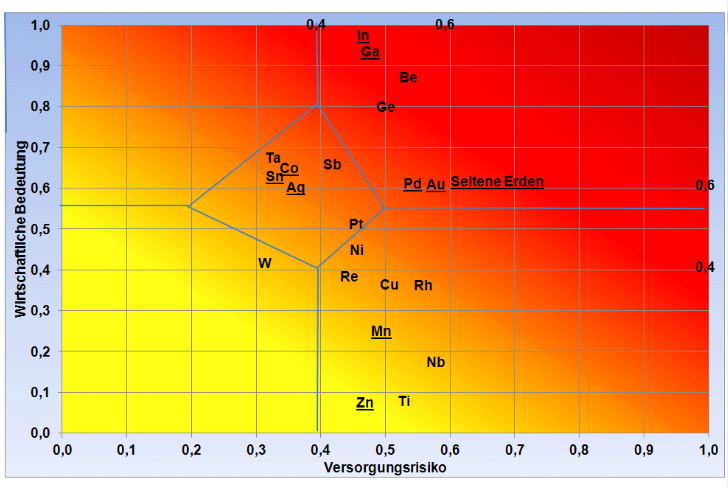
\includegraphics[width=\textwidth]{img/criticality}
    \caption{Economic significance vs. resource criticality, ~\cite{Studie} p.23 (\copyright~Rights belong to their respective owners)}%
    \label{fig:crit}
\end{figure}
%
\begin{table} [H]
    \centering
    \begin{tabular}{c c}
        \toprule
        Resource relevant metals & Contained in mobile phones (mg) \\ \midrule
        Gold & 30 \\ \midrule
        Silver & 305 \\ \midrule
        Palladium & 11 \\ \midrule
        Cobalt	& 6300 \\ \midrule
        Gallium	& 0.1 \\ \midrule
        Indium	& 2.4 \\ \midrule
        Tin	& 648 \\ \midrule
        Neodymium & 120 \\ \midrule
        Yttrium	& 0--0.01 \\ \midrule
        Tantalum & 0--2.4 \\ \midrule
        Antimony & No data \\ \midrule
        Beryllium & No data \\ \bottomrule
    \end{tabular}
    \caption{Resource-relevant metals in a smartphone,~\cite{Studie} p.45-63}%
    \label{tbl:crit}
\end{table}

Considering that demand from the world economy for these materials increases, the question of how much more rare materials can be mined from the earth without getting them back into circulation before an environmental collapse occurs, seems appropriate\footnote{Sander, Knut: Abfallwirtschaftliche Produktverantwortung unter Ressourcenschutzaspekte, p.7--25~\cite{Studie}}.

A silver lining is the fact that the telecommunication companies seem to have started to realize the gravity of the question raised above. Swisscom, the largest telecommunication company in Switzerland, created two programs to combat the problem that phones are hardly ever recycled. One of their programs, called ``Mobile Bonus'', offers their clients the possibility to sell their old phones back to Swisscom. The second program, called ``Mobile Aid'', lets people hand in their phones to Swisscom as a donation. The ``Réalise'' organization (dedicated to reintegrating welfare recipients) will then repair or recycle them, and all the profits made are donated to the SOS Kinderdorf foundation\footnote{Baur Roge, Der vergessene Schatz in unseren Schubladen, p.7--25~\cite{Swisscom}}. Despite the efforts of Swisscom and other actors, so far society seems to be unaware of the problem.

\section{Hackathon project}

We came up with a basic Ethereum-based token system that creates an economy that
rewards participants for interacting with their phones in an ecologically sustainable
way. We will first introduce the concept and try to justify our decisions, then
show some details of how the prototype was built.

\subsection{Concept (Anja)}
There are three different tokens in the system. A circulating token, called the SPCR Token (shorthand: SPC), a  second token that is used to exchange SPC into a Reputation Token, called the repair token (RPT), and the non-circulating reputation token (RT). For a schematic see figure~\ref{fig:cycles}.

Before we go into detail of how the system works, let us have a look at the three actors of the system. First, we have the telecommunication company where you can get a subscription for your mobile phone and recycle old ones (that don't get upcycled through the system). Then we have the ``repairperson'' who is a volunteer and offers his repair service (subsequently called ``repair guy'' for convenience). The repair guy is also a prosumer\footnote{A combination of a consumer and a producer}, as all actors apart from the telecommunication company. Those prosumers can offer repair services but also partake in the system as regular consumers.

There are a few different ways the tokens can be generated or used. Upon registering with the platform, a user is granted a certain amount of SPC to start with. A prosumer can get SPC by inviting new members into the network, which helps to expand the network and to reach more people (a typical referral system). A core mechanic is also getting  SPC by recycling old phones or collecting phones for recycling or reselling  as a service. When giving a repair guy an assignment to repair a phone, SPC can be earned by buying parts necessary for the repair (with real-world money) that are given to the repair guy, so he can do the repair. Lastly, SPC is transferred when ``reselling'' a phone in the system.

\begin{figure}
    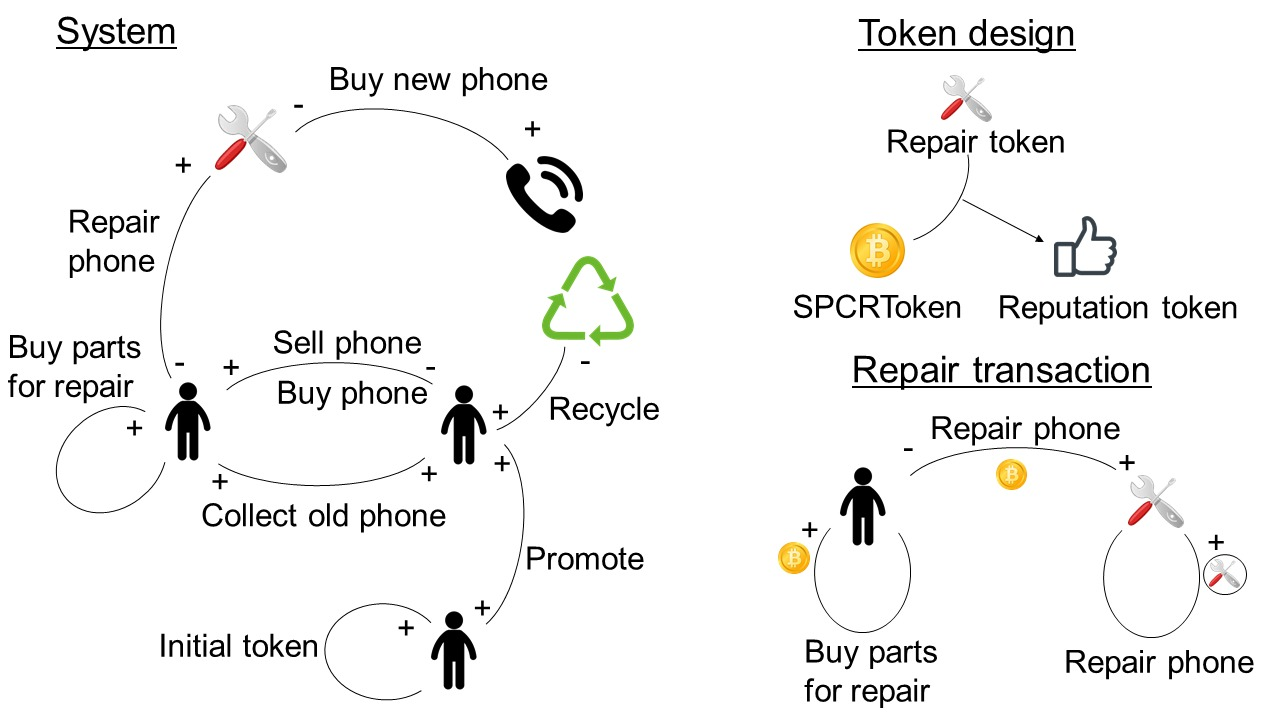
\includegraphics[width=\textwidth]{img/cycles.jpeg}
    \caption{Schematic of the SPCRT system}%
    \label{fig:cycles}
\end{figure}

So how can these different tokens now be used within the system? A prosumer can offer his phone for sale in exchange for an individually defined amount of SPCs to another prosumer. So, the SPC gets transferred from one prosumer to the other. The selling prosumer, of course, can be a repairing guy who bought older phones beforehand and then repaired or refurbished them, or someone who just got a new phone and wants to sell the old one.

If a prosumer wants his phone to be repaired, he or she can go to the platform to find the closest repair guys and get into contact with them (the repair guys would enter the location their office (for example) on the platform). He then can describe the problem to the Repair Guy or in special cases also bring it by for a short analysis of an unknown problem. The Repair Guy in return can communicate to the prosumer what kind of parts he needs for this job, in case he accepts the job as well as the expected amount of SPCs he wants in return. The prosumer then can launch a smart contract which the repair guy needs to confirm. After this, the prosumer buys the replacement parts (not with SPCs, in the real world) himself or organizes them in some other form. This generates him some additional SPCs. He then gives the phone and the parts to the repair guy who repairs the phone and returns it. The prosumer, after receiving the fixed or renewed phone, can confirm this and with this automatically initialize the actual SPC transfer. The repair guy receives, apart from the SPC, additional repair tokens. With these repair Tokens and some SPC Tokens he can create a reputation token which reflects his skill and overall customer satisfaction. With the SPCs it is also possible to get a discount on subscription from the telecommunication company. This should be an incentive for the repair guy for offering his skills. How much the discount should be, needs to be negotiated with the telecommunication company first. The last process is the collecting phones from others and recycling them. In this process a prosumer gives away his phone to another prosumer who collects them and already gets a certain amount of SPCs for this. When the collector recycles the mobile phones the prosumer who gave away the phone only gets half of the SPCs he would have gotten for recycling, and the other half goes to the collector. If the mobile phones are resold, the prosumer who gave away the phone gets a quarter and three quarter are for the collector. If the phone is from a person not registered to the network, the collector gets all the SPCs.

To add some further explanation to the repair tokens, the reason why the repair token were introduced is to prevent creating reputation of prosumers which do not offer a service and somehow try abusing the reputation system as the reputation should represent the number of completed repair jobs of a repair guy.

\subsection{Implementation}

\subsubsection{Contract (Philippe)}
The Smart Contract that was used in the project is a basic, minimal implementation of an ERC20\footnote{ERC20 specification~\cite{vogelsteller20erc}} compliant token contract. The ERC20 compliance is not directly relevant for the purpose of this token system, but with future extensions in mind, it could be beneficial to be able to trade it with other kinds of tokens. It also gives us better tool support, such as integration in Etherscan or Metamask.\\
%
\begin{lstlisting}[
    language=Solidity,
    caption=Smart contract function for introducing a new participant,
    label=lst:intro
]
/**
 * A user is introduced to the system
 */
function introduction(address referrer) public {
    spcrtBasic[msg.sender] = initalToken;
	spcrtBasic[referrer] = spcrtBasic[referrer].add(referralReward);
	_totalSupply = _totalSupply.add(initalToken.add(referralReward));
}
\end{lstlisting}
%
Listing~\ref{lst:intro} shows one of the extensions of the ERC20 contract we implemented: A function that facilitates introducing new participant with a referral system. An initial ``allowance'' of tokens is given to the new participant and the referrer is given a referral reward. Note that for a real system, much more security needs to be implemented. At the moment, there are no precautions that prevent abuse whatsoever. For the full contract, please refer to listing~\ref{lst:contract_full} in the appendix.

\subsubsection{Website (Raphael)}

Even though the Smart Contract is the core of our system, it's worthless without an interface where a casual user can interact with it. Instead of an app or native application we chose a website (see figure~\ref{fig:recycle_web} and~\ref{fig:main_web}). There are several reasons for that, the most important being flexibility. With a website, we get free cross-platform capability, whereas native applications are usually highly unportable. Our website will run in any modern web browser, even on mobile\footnote{As long as the Metamask plug-in is available}.

\begin{figure}[H]
    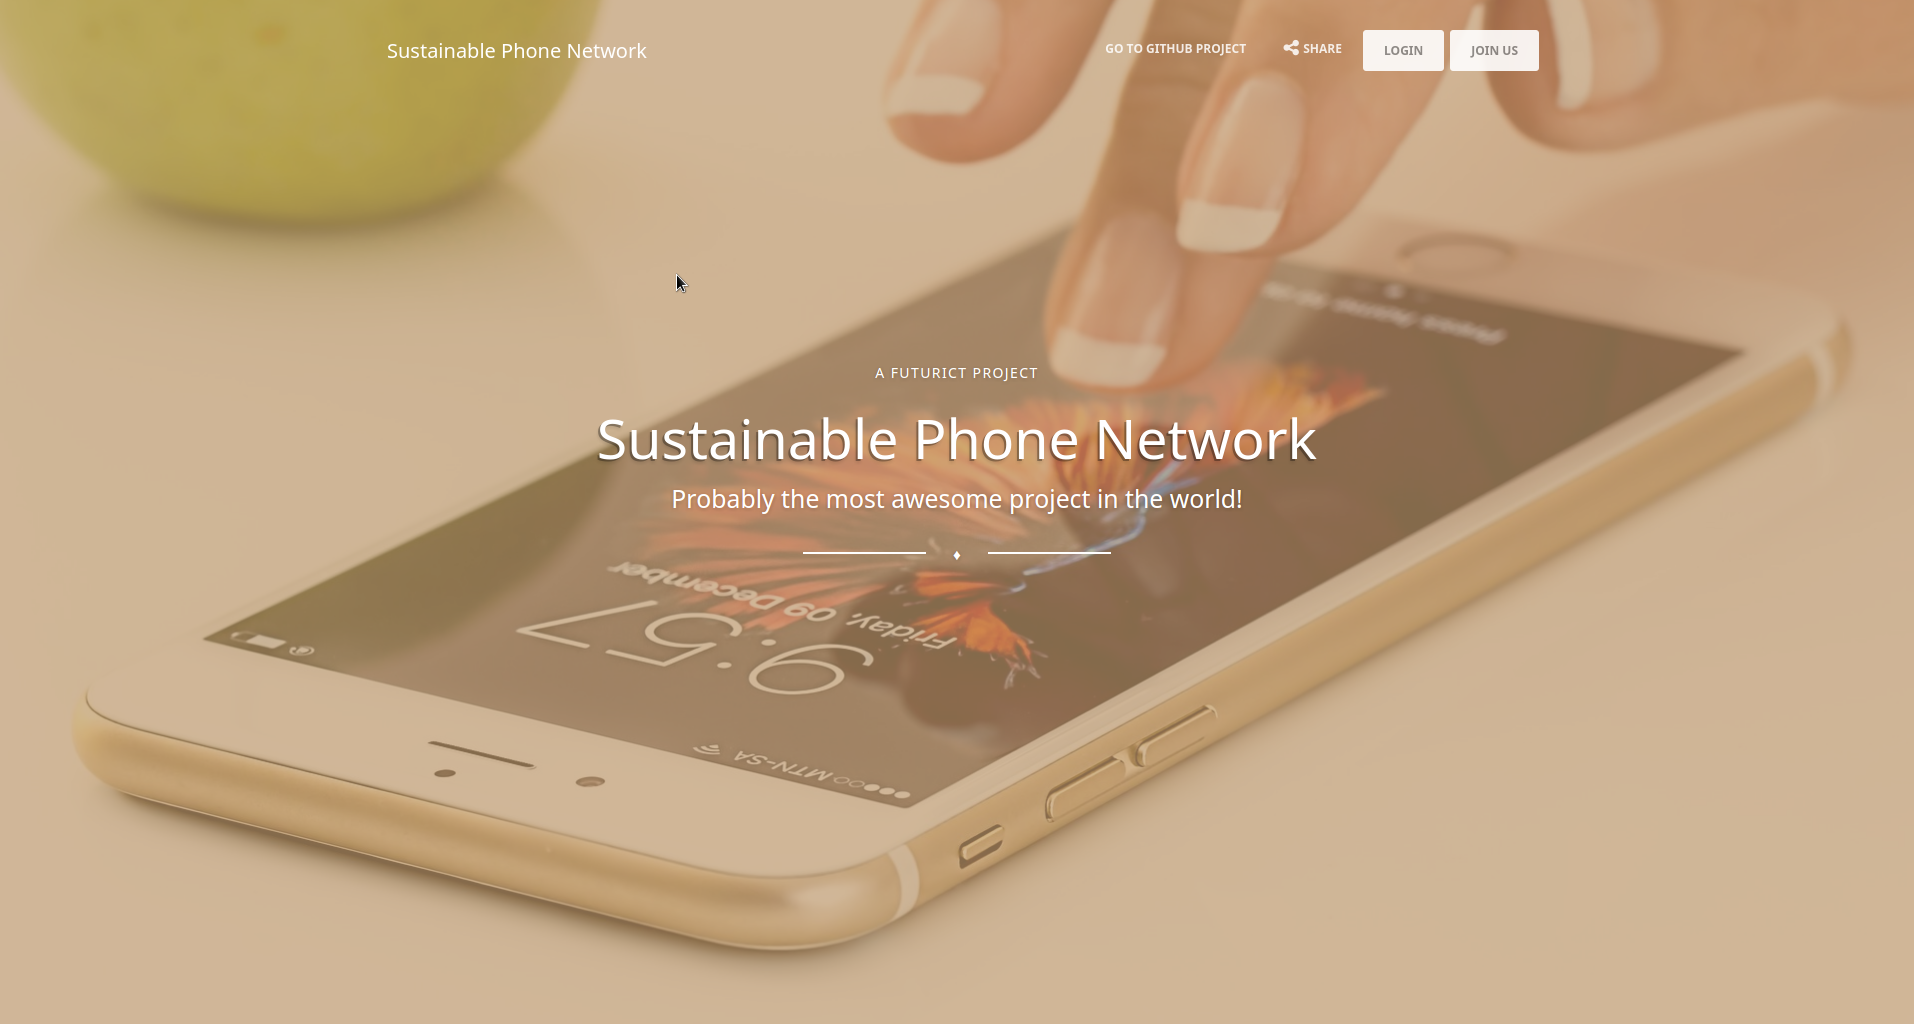
\includegraphics[width=\textwidth]{img/main_web}
    \caption{Website landing page}%
    \label{fig:main_web}
\end{figure}

The second big advantage is that the user does not have to download and install some software and is thus bound to a certain device, but instead can use any device (even public computers), by opening the website, logging in with his/her credentials.

The website in its current form relies on the third party extension ``Metamask''. Metamask makes transactions on Ethereum possible without having to sync a full node, by providing access to information on the blockchain with a web API. While very convenient, we believe this is a conflict in the core idea of Ethereum (having a fully decentralized network with no trusted third parties), and therefore would like to replace this with a better solution for a real product.

As the website interface, we chose a modern and user-friendly UI. At the start, you can either create a new account or log in if you are already registered. By doing so you end up on the dashboard, where the main user interaction takes place. The dashboard consists of the main page and the repair, recycle, and resell transfer forms. On the main page you can see all the basic information such as the number of tokens that are currently in your possession. Furthermore, you can choose which account you want to use to make the transaction. We added this functionality because there are probably parents with children too young to understand the system who also want to register their children. So instead of creating separate logins, the parents can add the children's account to their dashboard. On the repair page the user is able to make the transaction when a phone was repaired and also to find locations of repair guys around his/her location and how to contact them. On the recycle page there is a map of recycling facilities where the user can bring his/her phone to.

\begin{figure}[H]
	\fbox{%
		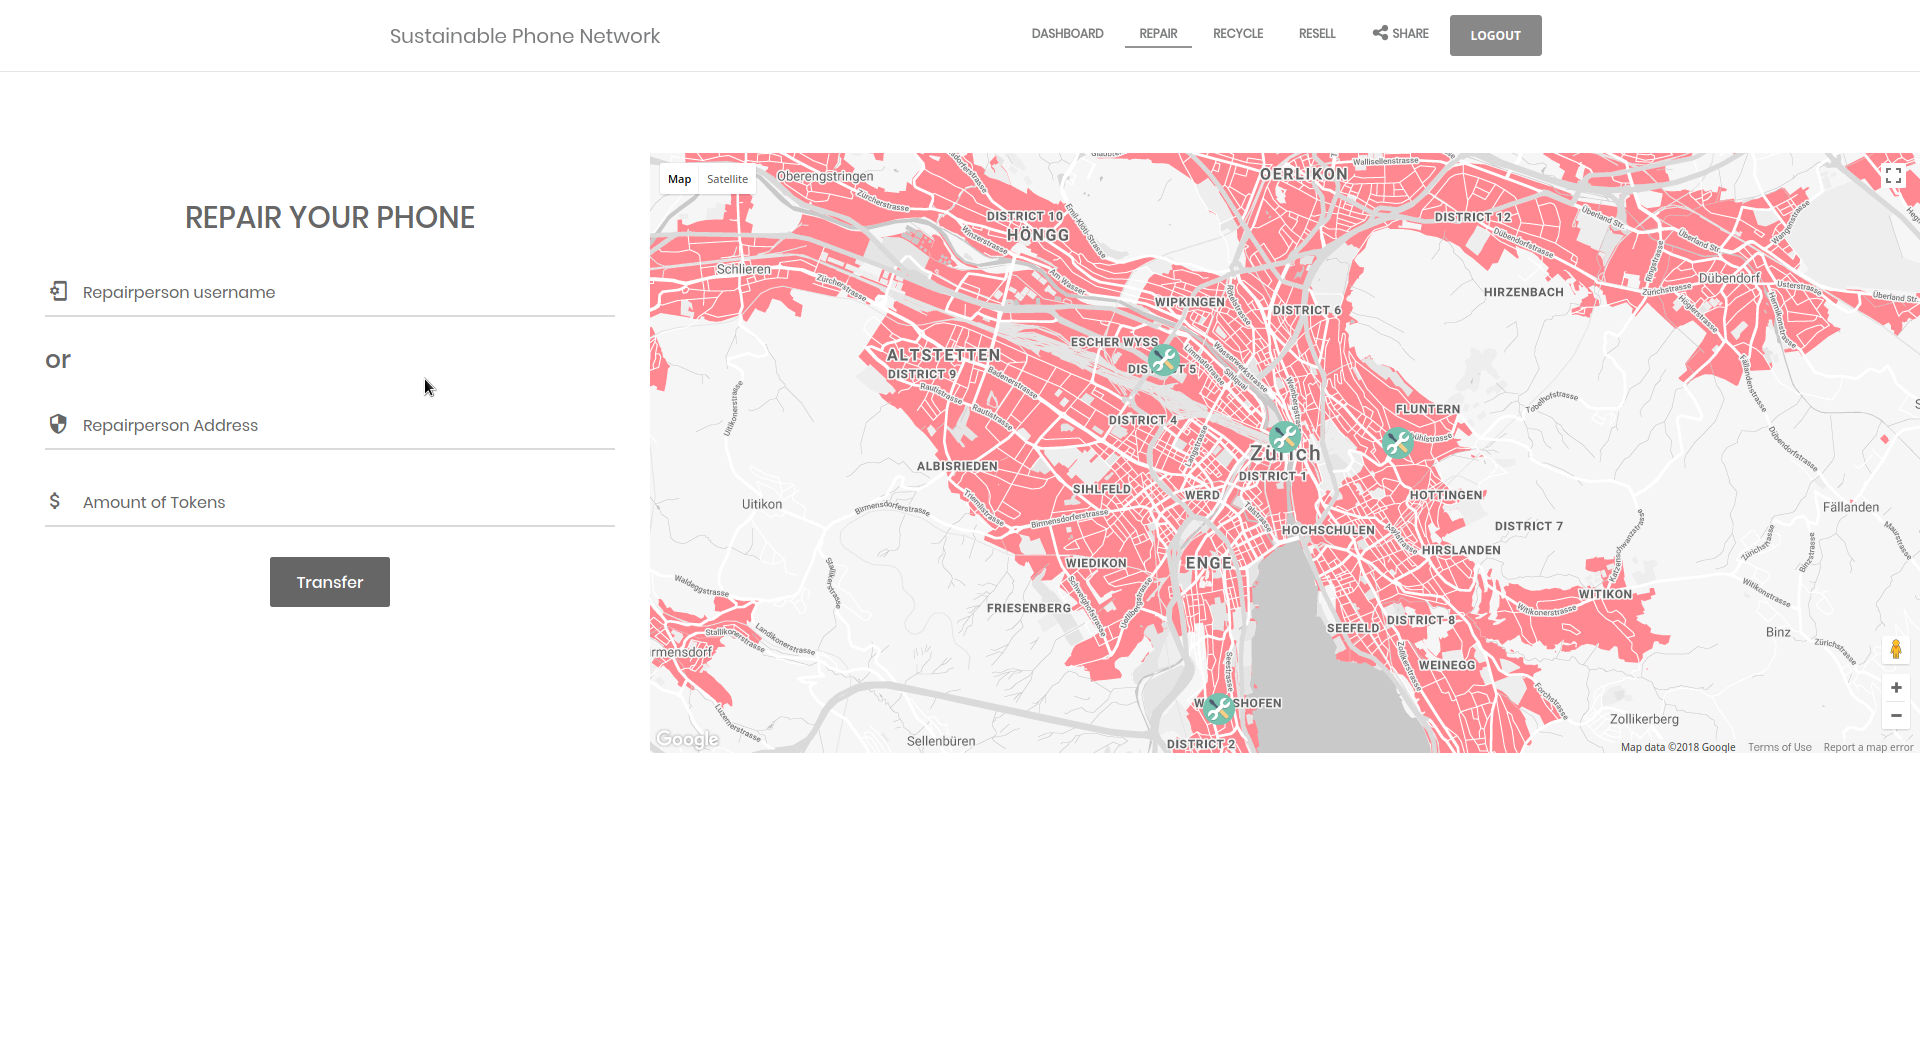
\includegraphics[width=\textwidth]{img/recycle_web}
	}
    \caption{Recycling page on the dashboard}%
    \label{fig:recycle_web}
\end{figure}

In addition to this, there is also a basic validation form. By recycling your phone the user receives a validation code which then can be entered in the validation form to enable the transaction of tokens to the user's account. This very basic measure is in place to prevent abuse by not allowing users to just click the ``recycle'' button as often as they want (ideally only once per recycled phone). Lastly, there is a ``resell'' page, where a transaction consisting of one participant selling his/her phone to another for some amount of token can be made.

\subsubsection{Analysis (Benjamin)}

An onerous portion of the project was deciding on how many tokens each of the incentives should return and to plan how they would be used from the prosumers. Since the system is not perfectly cyclic, it should be made sure all the tokens that are created can be burnt so no pools should form. In other words, it is assumed that the end goal of the token will be to be used on repairs or bonuses from the company, and in the meantime, they create a secondhand mobile phone market for people with old phones to trade.

Reviewing the four different token creation tasks, there is a certain uniqueness to some of them, specifically ``Buying parts for repair'' and ``Recycle'', meaning they contain a certain spurious component and only occur every so often. Imagine the average user has around X phones accumulated from previous years, once he recycles all his phones the next recycling phone event will not be so soon. However, these two tasks are the most compelling ones to promote good behavior, since they are critically important for the health of the environment as they produce recyclable material and, as stated earlier, most people do not recycle their mobile phones. There needs to be a balance between the rareness of an event, the initial offering of tokens, and the incentive for the user to use the ecosystem posterior to the initial bootstrap.  Taking all this into consideration, the distributions shown in table~\ref{tbl:mint_evt} and table~\ref{tbl:tok_burn} are adopted, explained further in the following paragraph.

\begin{table}[H]
    \centering
    \begin{tabular}{c c}
        \toprule
        Token Minting Event & Token Minted \\ \midrule
        Introduction the platform & 2 \\ \midrule
        Promoting the platform to other users & 1 \\ \midrule
        Buying parts for the repair & 8 \\ \midrule
        Recycling & 4 \\ \bottomrule
    \end{tabular}
    \caption{Token minted by the events}%
    \label{tbl:mint_evt}
\end{table}

\begin{table}[H]
    \centering
    \begin{tabular}{c c}
        \toprule
        Token Burning Event & Token burned \\ \midrule
        Upgrading reputation & 2 \\ \midrule
        Bonus from company& 5 \\ \bottomrule
    \end{tabular}
    \caption{Token burned by the events}%
    \label{tbl:tok_burn}
\end{table}

The reasoning behind this previous distribution follows the subsequent pattern of thought of how we believe users will join and use the ecosystem. First of all, once the platform is opened, users will register and get 2 tokens each, which is a way to airdrop tokens in order to bootstrap the system for people to be able to enter the market. Secondly, users will gather all their old mobile phones they have lying around home and go deposit them in an official spot, for helping in saving the environment we will reward them by giving them 4 tokens for each phone recycled. In this case, we had to balance the uniqueness of this event with the initial bootstrap. Considering it is quite possible that most users have many old phones lying around, overflowing and inflating the system with many tokens needed to be taken care of. However, it should be balanced with a high enough incentive for the experienced user to use the ecosystem to claim his tokens when he needs to change his current phone, hopefully after many years of use. Adding to all this, we needed the incentive for recycling to be lower than repairing the phone since repairing expands the lifespan of the user's current phone. Considering all the above we came up with 4 tokens to recycle each phone, this way there is not much inflation at the start of the project and once the user decides to change his phone, by just inviting a friend he will be able to receive a bonus from the company and keeps using the system. Thirdly, users that want to get easy bonuses will invite their friends with the proper referral link and get one token for each user that accepts their invitation. This would conclude the initialization of the system, as stated earlier, the easier, and more frequent it is to do a task the lesser tokens they receive for it. Once inside the system, the user can either buy old mobile phones or use their tokens to repair their current phone or use their tokens to get a discount or other benefits from their phone company.

Let us pay more attention to the repair part. As stated earlier, this is one of the most important tasks a user can do to be environmentally friendly. If a user needs to change a part of the phone and buys the part, he will receive 8 tokens. The logic behind this is twofold: first to reward the customer for his good deed and secondly for him to be able to pay the repairman a fair price for his repair. Since the reputation costs 2 tokens to upkeep, the minimum a repairman would then take would be 2 and, optimally, a fair price would be 3 tokens so the repairman has an incentive to repair other than to upkeep his reputation. In this optimal pricing of 3 tokens for repair\footnote{This is our model's optimal price, however, the users are free to ask whatever they want.}, the user would be able to use his repairing service and also get a bonus from the company and would have an incentive to continue using his phone.

Another point of having a reputation system for the repairman's is because otherwise the repairman's had an unfair advantage over the rest of the users. They would amass a large amount of tokens and create pools where the cycle of the token would break. This still happens, if we look at the simulation of the system at figure~\ref{fig:analysis}, we can still see how the repairman's have a larger amount of tokens compared to normal users. A naive thing to do would be to raise the amount a reputation point costs, however by doing so, the repairman's would just raise the price of the repair to match the cost of the reputation token.

Finally, the bonus from the company is given by thinking of certain possible and frequent combinations of minting events. For example, as stated before, an advanced user of the system wants to recycle his current phone after many years of use, by recycling the phone he will only need to invite one person in the system before he is able to receive a perk from the company (4 + 1 tokens). Another example is a user that just came arrived, he would easily be able to get one perk just by joining and recycling a phone (4 + 2 tokens). In previous paragraphs, we also gave an example how a user that wants to repair his phone would be benefited.

Following this distribution, we simulated how the end distribution of tokens would end up hoping that no malicious actors try to interfere or exploit the system. To do this, 10,000 users are simulated. 500 of them are marked as repairmen. We simulate random values according to a few selected probability distributions that we think match correctly each task. In other words, random values are created according to a few parameters to create the distribution of a normal user versus a repairman for comparison purposes. For details, see the R source code in the appendix.

To model the number of referrals that new user would bring, a Poisson distribution with mean 3 is employed, representing that every new user would bring three new users which seems reasonable enough. For the distribution of accidents and therefore repairs, zero-inflated Poisson distribution is used, which always works well with accidental data, as we usually have large amounts of zeros and people who are frequently involved in accidents are rather rare.\footnote{Dominique Lord et al, Poisson, Poisson-Gamma and zero-inflated regression models of motor vehicle crashes: balancing statistical fit and theory~\cite{Statistics}}' To simulate the amounts of old phones used, a Gamma distribution is assumed to model the shape of how we think the distribution is. The amount of tokens a repair transaction would ask is also modeled with a ZIP, although with a few modifications. First, we move the add to the distribution 2, so instead of being a zero-inflated it will be a ``two inflated'' the reasons for this are stated earlier for the reputation costs. Secondly modifying the parameters of the distribution we can get almost the same amount of people that will ask for 2 tokens and people that will ask for 3 tokens, afterward a common Poisson distribution is followed. We remind the reader that this is obviously taking many assumptions, and as the users of the system are free to do whatever they please, we can't make any guarantees on correctness, for the sake of argument we are making many conjectures which would need real data for a validity model. 

See figure~\ref{fig:analysis} for a plot of the simulation results.

\begin{figure}[H]
    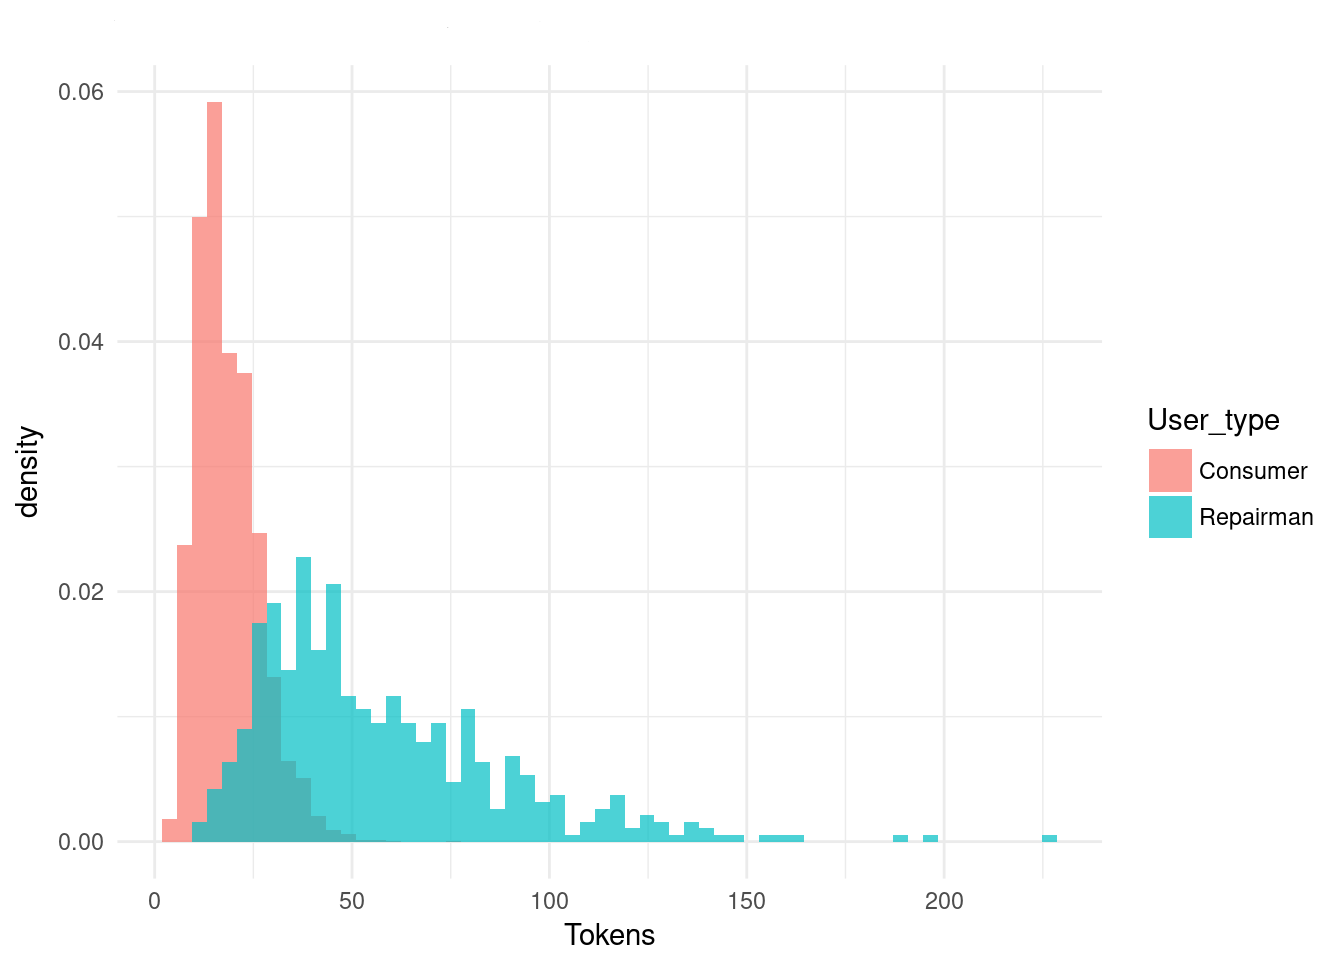
\includegraphics[width=\textwidth]{img/analysis}
    \caption{Distribution of tokens among users and repairman}%
    \label{fig:analysis}
\end{figure}

Our simulation right now lacks the option to spend the tokens for a discount on phone contracts, however this does not matter since the whole purpose of the simulation was to see how far apart the normal prosumers were in comparison to the repair guys without the possibility to remove tokens from the system. We were slightly concerned that the repair guys would amass a large amount of tokens. This does actually happen in our simulations, however not as much as we previously assumed: on average the repair guy will hold three times as many tokens as the unskilled user. Introducing a way for the repair guys to spend their tokens outside the system should even out that gap even more. In conclusion, theoretically the token life cycle should also work on a longer term.

\subsection{Open questions \& difficulties (Anja and Philippe)}
At the end of the week some open questions and difficulties needed to be faced.  One of the question and probably one of the crucial ones was if the telecommunication companies would be willing to cooperate  with our system as in case they wouldn't the Repairing Guy maybe will not have enough incentive to offer his service to the network. Concerning the telecommunication company, their incentive why they should give a discount is because with this they first can reduce their costs for repairing services as they could outsource it to some extent. Another reason is as they get more phones back which first of all helps their image and secondly, they can resell them again which as in the intro part said seems to be thoroughly interesting for them.

Then of course even with the support of the telecommunication companies, the insecurity remains if there will be enough prosumers who would like to offer their repairing services or even have the required skills. With the offered discount from the telecommunication companies it is hoped to create a big enough incentive. We strongly believe that there will be no lack of prosumers who would like to use the offered service as they get a repaired phone for free actually.

Finally, there are also some implementation difficulties or technical open questions. Of course, it could be assumed that trust is enough and nobody will abuse the vulnerabilities of the current implementation of the system. Therefore a system of checks needed to be implemented.

The plan was to expand the contract in a way that would allow certain validation checks to be performed. Currently, it's possible to cheat the system be just issuing the recycling function multiple times to obtain an infinite number of tokens. To mitigate this the idea was using an IoT box that can detect whether an object is a phone. If the object is indeed a phone the box should trap it inside and issue a validation code that can be used to gain the tokens for the recycling action.  To validate obtaining tokens for collecting phones there were two ideas:

\begin{itemize}
    \item Relying on trust. This means that the original owner of the phone
        confirms that the phone was collected from him. However, this could
        potentially be exploited because two people could just infinitely often
        collect each other's phones.
    \item Recording the ``collection transactions'' by maintaining an append-only
        list (maybe on IPFS) in the form of a Merkle-hash tree where the
        root-hash could be stored on the blockchain to ensure integrity. To
        make a ``collection transaction'' the IMEI number of the phone would be
        recorded into the database so the same phone could not be collected
        multiple times.  The problem with this method is that IMEI numbers can
        easily be forged and thus two people can still collect virtually
        infinitely many tokens by creating arbitrary IMEIs. One possible
        solution could be the usage of an app that verifies the IMEI directly
        on the phone, but this would make it impossible to obtain tokens for
        broken phones and it would also make the token system harder to use.
        In conclusion, one must admit that for the sake of accessibility it
        makes sense to waive this security mechanism and solely rely on trust.
\end{itemize}


\subsection{Challenges (Anja)}
There are some challenges concerning the further development of the idea. Initially, the idea was to include in the system all kind of electronic devices so that the repair guys instead of getting a discount from the telecommunication company could use their SPCs for other repairing services offered by other prosumers. Due to the limited time of this course, the concept was restricted only to phones as these so far still have one of the worst recycling rates from electronic devices as stated in the introduction. Nevertheless, this system could be expanded to other electronic devices as laptops, televisions, microwaves etc. However, it probably is better to create subsystems similar to the one for the phone for each device or set of similar devices and then just introduce a token system where the different tokens could be used in the other subsystems or could be traded with the other tokens.

If we think even further the system could be expanded even to other parts of economy as for example the textile industry where repair could be even easier sometimes than for an electronic device. Services like sewing, knitting or customizing clothes could be offered. We believe our system could be applied to various different products.

Generally speaking a transformation from our current consumer society back to the preserving society of our grandparents, which is linked to a transition from a purely capitalistic economy to a more shared and social economy, could be favorable for our world and our future.

\section{Possible outcomes and changes for society (Anja)}

How could our society change with this system? First of all our system definitely represents a threat to the currently existing commercial mobile phone repair shops. Maybe a coexistence could be established between these two where the repair shop acts as repair part provider for the prosumers or as a equipment and expertise renting system for the repair guys. In this way, existing infrastructure could be preserved and used for the system.

Even though in the beginning, the system would only get implemented with mobile phones, this could lead to a sensitization of the people and therefore could also simplify the expansion of the system to other electronic devices. This generally should raise the awareness of the people for the resource scarcity our world is facing. People should start to acknowledge and appreciate the true value of phones and treat them respectively instead of perceiving them as a status symbol.

There are several final goals of the whole idea. One of them is to increase the circularity of the resources used in phones as they get recycled. Another one is to encourage elongated use of mobile phones with selling and buying old phones or repairing them. Therefore, ideally all phones should be repaired if feasible instead of being recycled. With this, the mobile phone should get a second life. Both of the aforementioned goals should help to decrease or stagnate the demand of the resource relevant materials, as they were called in the introduction.

There could also be some potential changes for the telecommunication companies or even for the mobile phone producers. As already mentioned shortly in the open question and difficulties part, telecommunication companies could outsource parts of their repairing service to the repair guys for discounts for example. They could also start offering additional subscriptions without new mobile phones. This is believed to be an advantage in the sense of the costs that can be saved as the telecommunication companies don't need to buy the mobile phones from the mobile phone producers to offer them cheaper to the customer. This also could help stop the hype of getting a new mobile phone every year. The change in mentality of the people concerning the mobile phones could lead to a change in paradigm of the mobile phone producers. Instead of even cheaper and even less repairable, to a more modular and a more sustainable design which also could allow to replace individual parts.

\printbibliography%

\pagebreak
\section*{Appendix}

\begin{lstlisting}[language=R,caption={Simulation},captionpos=b,label=lst:sim]
library(gamlss.dist)
library(ggplot2)

set.seed(1714)

mint <- c(2,1,8,4) # inicialization, promotion, repairs, recylcle

sim <- vector(length = 10000)
# lets create 500 random repair people
repair_id <- sample(1:10000, 500)
j <- 1

for(i in 1:10000){
  if(i %in% repair_id){
      aux <- rZIP(1, mu = 0.80, sigma = 0.5) # number of accidents/repairs
      sim[i] <-sum(mint*c(1,
                      rpois(1,3), # generate random poison with mean 3
                      aux,
                      round(rgamma(1, 3, 1)) # round a gamma distribution with rate 3 and scale 1
                      ) + sim[i]
  )

  } else {
      aux <- rZIP(1, mu = 0.80, sigma = 0.5) # number of accidents/repairs
      sim[i] <-sum(mint*c(1,
                      rpois(1,3), # generate random poison with mean 3
                      aux,
                      round(rgamma(1, 3, 1)) # round a gamma distribution with rate 3 and scale 1
                      )
  )
  }
  # if we need to repair
  if(aux != 0){
    # Who repaired
    who <- sample(repair_id,1)

    j <- j + 1
    aux2 <- rZIP(1, mu = 2, sigma = 0.01) + 2 # price of repair
    sim[i] <- sim[i] - aux2*round(aux) # amount payed and substracted user
    sim[who] <- sim[who] + aux2*round(aux) - 2*round(aux) # amount payed to repairman
  }
}

df <- data.frame(Tokens = sim, User_type = "Prosumer", stringsAsFactors = F)
df$User_type[1:10000 %in% repair_id] = "Repairman"


ggplot(data=df, aes(x=Tokens, y = ..density.., fill = User_type)) +
  geom_histogram(bins = 60, alpha = 0.7, position = "identity") +
  theme_minimal() +
  ggtitle("Density distribution of tokens among users vs. repairmans") +
  guides(fill=guide_legend(title="User type")) +
  ylab("Density")
\end{lstlisting}

\begin{lstlisting}[
    language=R,
    caption={Graph generation},
    captionpos=b,
    label=lst:graphgen
]
knitr::kable(t(summary(df$Tokens[df$User_type == "Repairman"])),
    caption = "Summary statistics for the Repairman class")
knitr::kable(t(summary(df$Tokens[df$User_type == "Prosumer"])),
    caption = "Summary statistics for the Prosumer class")
\end{lstlisting}

\begin{lstlisting}[
    language=Solidity,
    caption={Full SPC smart contract},
    captionpos=b,
    label=lst:contract_full
]
pragma solidity ^0.4.19;

import "./SafeMath.sol";
import "./ERC20Interface.sol";
import "./Owned.sol";

/**
 * SPCRToken System implementation
 */
contract SPCRToken is ERC20Interface, Owned {
    using SafeMath for uint256;

    string public constant name = "SPCRToken";
    string public constant symbol = "SPC";
    uint8 public constant decimals = 18;

    uint256 private initalToken = 4;
    uint256 private recycleReward = 2;
    uint256 private referralReward = 1;
    uint256 private collectionReward = 1;

    uint256 public _totalSupply;

    mapping (address => mapping (address => uint256)) allowedSpcrtBasic;

    mapping (address => uint256) spcrtBasic;
    mapping (address => uint256) spcrtReputation;

    // repair transaction (sent by guy that wants repair done)
    function transferRepair(
        address repairGuy,
        uint256 tokens
    ) public returns (bool success) {
        spcrtBasic[msg.sender] = spcrtBasic[msg.sender].sub(tokens);
        spcrtBasic[repairGuy] = spcrtBasic[repairGuy].add(tokens);

        // update repairGuy reputation
        spcrtReputation[repairGuy] = spcrtReputation[repairGuy].add(1);

        Transfer(msg.sender, repairGuy, tokens);
        return true;
    }

    // query reputation of an address
    function getReputation(address addr) public view returns (uint256 rep) {
        return spcrtReputation[addr];
    }

    /*
     * ERC20 Interface implementations
     */

    function totalSupply() public constant returns (uint) {
        return _totalSupply  - spcrtBasic[address(0)];
    }

    function balanceOf(address tokenOwner) public constant returns (uint balance) {
        return spcrtBasic[tokenOwner];
    }

    function allowance(address tokenOwner, address spender) public constant returns (uint remaining) {
        return allowedSpcrtBasic[tokenOwner][spender];
    }

    function transfer(address to, uint tokens) public returns (bool success) {
        spcrtBasic[msg.sender] = spcrtBasic[msg.sender].sub(tokens);
        spcrtBasic[to] = spcrtBasic[to].add(tokens);
        Transfer(msg.sender, to, tokens);
        return true;
    }

    function approve(address spender, uint tokens) public returns (bool success) {
        allowedSpcrtBasic[msg.sender][spender] = tokens;
        Approval(msg.sender, spender, tokens);
        return true;
    }

    function transferFrom(address from, address to, uint tokens) public returns (bool success) {
        spcrtBasic[from] = spcrtBasic[from].sub(tokens);
        allowedSpcrtBasic[from][msg.sender] = allowedSpcrtBasic[from][msg.sender].sub(tokens);
        spcrtBasic[to] = spcrtBasic[to].add(tokens);
        Transfer(from, to, tokens);
        return true;
    }

    /**
     * Mint coins for recycling
     */
    function mintRecycle() public {
        spcrtBasic[msg.sender] = spcrtBasic[msg.sender].add(recycleReward);
		_totalSupply = _totalSupply.add(recycleReward);
    }

    /**
     * A user is introduced to the system
     */
    function introduction(address referrer) public {
        spcrtBasic[msg.sender] = initalToken;
		spcrtBasic[referrer] = spcrtBasic[referrer].add(referralReward);
		_totalSupply = _totalSupply.add(initalToken.add(referralReward));
	}

    /**
     * Mint for collection mechanism
     */
    function mintCollection(address objReceiver) public {
        spcrtBasic[msg.sender] = spcrtBasic[msg.sender].add(collectionReward);
        spcrtBasic[objReceiver] = spcrtBasic[objReceiver].add(collectionReward);
        _totalSupply = _totalSupply.add(collectionReward.mul(2));
    }

    /**
     * Don't accept ethers
     */
    function () public payable {
        revert();
    }
}
\end{lstlisting}

\end{document}
